\section{Respuesta electromagnética de materiales plasmónicos}

En el artículo original de Mie \cite{mie1908metallosung} se emplea la solución a los campos EMs esparcidos para describir las propiedad ópticas de suspensiones coloidales de partículas esféricas de oro\index{Mie!solución de}. En sus cálculos, Mie asumió que la  respuesta electromagnética del oro en bulto, dada por los datos experimentales de la función dieléctrica $\varepsilon(\omega)$,\index{Función dieléctrica} era válida también para nanopartículas (NPs) cuyo radio fuera un orden de magnitud menor al de la longitud de onda de la luz que ilumina a la NP \cite{horvath2009historic}. A pesar de que la suposición de Mie es válida para los cálculos que publicó \cite{horvath2009historic}, en general la respuesta electromagnética de los materiales depende de sus dimensiones y a la nanoescala los efectos de superficie cobran relevancia respecto a los de bulto\footnote{Una diferencia en la respuesta EM de bulto respecto a la de NPs ocurre cuando el camino libre medio de los electrones libres de algún metal es mayor que las dimensiones de la NP, en este caso debe hacer una corrección que considere este efecto de superficie \cite{noguez2007surface}.} \cite{noguez2007surface,mendoza2014determination}, por lo que la función dieléctrica de bulto debe corregirse para NPs. 

Para corregir la respuesta EM  en bulto de materiales plasmónicos, se asume que su función dieléctrica corresponde a la suma de la respuesta de los electrones de conducción del material  $\varepsilon^{intra}(\omega) $, correspondiente a las transiciones electrónicas intrabanda, y con los electrones ligados  $\varepsilon^{inter}(\omega) $, correspondientes a las transiciones electrónicas interbanda\index{Función dieléctrica!interbanda}\index{Función dieléctrica!intrabanda} \cite{noguez2007surface}, es decir
%
	\begin{align*}
	\varepsilon^B_{exp}(\omega) = \varepsilon^{intra}(\omega) + \varepsilon^{inter}(\omega),
	\end{align*}
%
en donde $\varepsilon^B_{exp}(\omega)$ es la función dieléctrica de bulto, que se determina de forma experimental \cite{johnson1972constants}. Es posible considerar los efectos de tamaño en $\varepsilon^{intra}(\omega)$ empleando el modelo de Drude-Sommerfeld, el cual describe la función dieléctrica de un material en bulto con electrones de conducción a partir de asumir un gas de electrones libres \cite{gross2014festkorperphysik}. Al corregir el modelo de Drude-Sommerferd considerando los efectos de tamaño de la NP e introducir esta corrección en los datos experimentales del bulto, se construye una función dieléctrica apta para NPs y el cálculo de sus propiedades ópticas mediante la solución de Mie.\index{Drude-Sommerfeld!modelo de}

\subsection{Modelo de Drude-Sommerfeld}

 Para describir la contribución de los electrones de conducción en la respuesta EM del material $\varepsilon^{intra}(\omega)$ se emplea el modelo de Drude-Sommerfeld que, desde un enfoque clásico, es la solución a la ecuación de movimiento de los electrones libres en un material ante la presencia de un campo eléctrico externo oscilante \cite{gross2014festkorperphysik}. El efecto de un campo eléctrico externo $\vb{E}$ sobre los electrones libres de un material es un cambio en su posición, por lo que aparecen momentos dipolares $\vb{p}=q_e\vb{r}$; con $q_e$ la carga del electrón y $\vb{r}$ su desplazamiento.  El efecto neto en el material es una polarización $\vb{P} = n_v \vb{p}$, donde $n_v$ es la densidad volumétrica electrónica \cite{novotny2006principles}.  La respuesta óptica del material dada por el modelo de Drude-Sommerfeld, caracterizada por la función dieléctrica $\varepsilon_D(\omega)$, depende de $\vb{E}$ y $\vb{P}$ como \index{Electrón!libre}
%
	\begin{align}
	\vb{P} = n_v q_e \vb{r} =\varepsilon_0\qty(\frac{\varepsilon_D(\omega)}{\varepsilon_0}-1)\vb{E},
	\label{eq:PolarizationDrude}
	\end{align}
%
donde se asume que la polarización ocurre en la dirección del campo eléctrico \cite{novotny2006principles}. Si el material se encuentra ante la presencia de un campo eléctrico oscilante de la forma $\vb{E}_0 e^{-i\omega t}$, la ecuación de movimiento que obedece un electrón libre del material es \cite{kreibig1995clusters,gross2014festkorperphysik}\index{Drude-Sommerfeld!modelo de!ecuación de movimiento}\index{Ecuación!de movimiento de un electrón libre}\index{Ecuación!de movimiento de un electrón libre|seealso{Drude-Sommerfeld}}
%
	\begin{align}
	m_e^* \pdv[2]{\vb{r}}{t} +  \gamma \pdv{\vb{r}}{t} = q_e\vb{E}_0e^{-i\omega t},
	\label{eq:movementDrude}
	\end{align}
%
donde $m_e^*$ es \index{Electrón!masa eféctica del}la masa efectiva del electrón\footnote{La masa efectiva es el resultado de la interacción de un electrón con el potencial de la red cristalina que conforma al material, con los fonones de la red y con otros electrones en la red \cite{gross2014festkorperphysik}. } \cite{gross2014festkorperphysik} y $\gamma$ es la \emph{constante fenomenológica de amortiguamiento} \cite{kreibig1995clusters}, que es el inverso del tiempo promedio entre eventos de colisiones  de los electrones \cite{novotny2006principles,gross2014festkorperphysik}.  Al multiplicar la Ec.  \eqref{eq:movementDrude} por $n_v q_e$, resolverla con el \emph{Ansatz} $\vb{r} = \vb{r}_0e^{-i\omega t}$ y compararla con la Ec.  \eqref{eq:PolarizationDrude}, se obtiene la función dieléctrica tipo Drude: \cite{novotny2006principles,gross2014festkorperphysik}\index{Drude-Sommerfeld!modelo de}\index{Drude-Sommerfeld!modelo de!frecuencia de plasma $\omega_p$}\index{Función dieléctrica!tipo Drude}  \vspace*{-.75em}
%
	\begin{tcolorbox}[title = Modelo de Drude-Sommerfeld, breakable ]
	\eqhalf{\frac{\varepsilon_D(\omega)}{\varepsilon_0}= 1 - \frac{\omega_p^2}{\omega(\omega+i\gamma)},
	\label{eq:Drude}}
	\eqhalf{	\omega_p =\sqrt{ \frac{n_v q_e^2}{m_e^* \varepsilon_0}},
	\label{eq:wp}}
	\end{tcolorbox}\vspace*{-.75em}\noindent
%
con $\omega_p$, la frecuencia de plasma. La constante fenomenológica $\gamma$ depende de las dimensiones y geometría del material, por ejemplo, para un material en bulto, se emplea en la Ec. \eqref{eq:Drude} $\gamma=\gamma_\infty$, con $\gamma_\infty$ la constante fenomenológica de bulto  ---que se considera como una esfera de radio $a\to\infty$--- dada por \cite{kreibig1995clusters} \index{Drude-Sommerfeld!modelo de!constante fenomenológica de amortiguamiento de bulto $\gamma_\infty$}
%
	\begin{align}
	\gamma_\infty = \frac{v_F}{L},
			 \label{eq:gammaInf}	
	\end{align}
%
donde $v_F$ es la velocidad de Fermi\footnote{\index{Fermi!velocidad de}En un sistema con $N$ electrones, que obedecen el principio  de exclusión de Pauli, la energía de Fermi $E_F$ es la que corresponde al nivel energético ocupado ocupado con mayor energía, y está dada por $E_F = (\hbar^2/2m_e^*)k_F^2$, con $k_F$ la norma del vector de onda de Fermi \cite{gross2014festkorperphysik}.  Puesto que la velocidad de Fermi es $v_F = p_F/m_e^* = \hbar k_F / m$ y que para un gas de electrones libres $k_F=(3\pi n_v)^{1/3}$, se obtiene que para metales como el oro, plata o cobre,  $v_F\approx 10^{15}$ nm s$^{-1}$ \cite{gross2014festkorperphysik,ashcroft1976solid}. } del material a una temperatura dada y $L$ es el camino libre medio, que representa la distancia promedio que recorren los electrones entre eventos de colisiones \cite{gross2014festkorperphysik}.  

La frecuencia de plasma $\omega_p$ en el modelo de Drude-Sommerfeld delimita regímenes donde el material plasmónico se comporta como un metal o como un dieléctrico \cite{trugler2011properties}.  En la Fig.  \ref{fig:Drude} se grafican las funciones dieléctricas (gráfica interna) y los índices de refracción  (gráfica principal) modelados por una función tipo Drude [Ec. \eqref{eq:Drude}] con $\hbar\omega_p=4. 3$ eV [Fig.  \ref{sfig:Drude4eV}] y $10$ eV [Fig.  \ref{sfig:Drude10eV}], y $\hbar\gamma=0. 15$ eV.  En estas gráficas se observa que $\Re[\varepsilon(\omega)]<0$ para $\omega<\omega_p$, por lo que al sustituir el índice de refracción en la expresión de una onda plana propagante se obtiene una onda evanescente, es decir, la onda plana no penetra el material y es reflejada: el material presenta una respuesta metálica.  Para $\omega>\omega_p$ se cumple que $\Re[\varepsilon(\omega)]>0$ y $\Im[\varepsilon(\omega)]\approx 0$, por lo que el índice de refracción, en dicho régimen, se comporta como el de un  material transparente. \index{Onda!evanescente}

	\begin{figure}[h!]\centering\hspace*{-1.5em}
	\begin{subfigure}{.01\linewidth}\caption{}\label{sfig:Drude4eV}\vspace{3.75cm}\end{subfigure}
	\begin{subfigure}{.45\linewidth}\hspace*{-1.3em}
	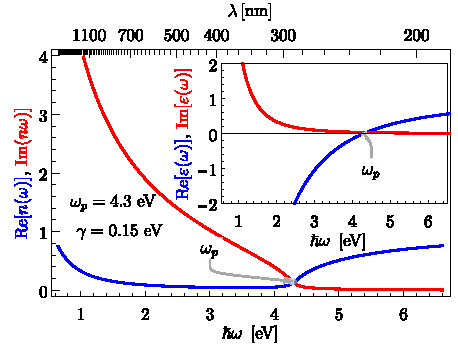
\includegraphics[scale=1]{1-Teoria/figs/1-4-varepsn4eV.pdf}
	\end{subfigure}
	\begin{subfigure}{.01\linewidth}\caption{}\label{sfig:Drude10eV}\vspace{3.75cm}\end{subfigure}
	\begin{subfigure}{.45\linewidth}\hspace*{-1em}
	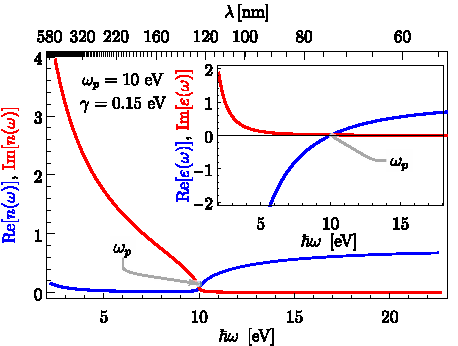
\includegraphics[scale=1 ]{1-Teoria/figs/1-4-varepsn10eV.pdf}
	\end{subfigure}\vspace*{-.7em}
	\caption{ Índice de refracción (gráfica externa) y función dieléctrica (gráfica interna) del modelo de Drude-Sommerfeld para las frecuencias de plasma \textbf{a)} $\omega_p=4. 3$ eV y \textbf{b)} $\hbar\omega_p=10$ eV; ambos casos con $\hbar\gamma=0. 15$ eV, como función de la energía.  En el marco superior se observa su dependencia en longitud de onda $\lambda$. }\label{fig:Drude}
	\end{figure}	

\subsection{Corrección por tamaño para partículas esféricas}

La corrección de la función dieléctrica para NPs esféricas a partir de la función dieléctrica de bulto $\varepsilon_B^{exp}(\omega)$, obtenida mediante métodos experimentales, consiste en la modificación de la constante fenomenológica de amortiguamiento en el modelo de Drude-Sommerfeld\footnote{También es posible hacer una corrección de tamaño en la contribución interbanda de la función dieléctrica considerando la densidad de estados sin embargo, para los datos experimentales de \cite{johnson1972constants}, esta corrección para partículas esféricas es apreciable para NPs con radios menores a $2$ nm \cite{mendoza2014determination}.}, dado que ésta depende del camino libre medio de los electrones $L$ y debe modificarse cuando el radio de las NPs $a$ es menor a $L$ \cite{kreibig1995clusters}. Por ejemplo, para metales típicos  como el oro y la plata, a frecuencias del espectro visible y a una temperatura de $273$ K, el camino libre medio de los electrones libres para el oro y la plata es  de $56$ nm  y $42$ nm, respectivamente\footnote{Cálculos a partir de los datos obtenidos de las tablas 1.3 y 2.1 de \cite{ashcroft1976solid}, donde $v_F^{Au} = 1.40\times 10^{15}$ nm s$^{-1}$ y $v_F^{Ag}=1.39\times 10^{15}$ nm s$^{-1}$.\index{Fermi!velocidad de}}, por lo que para NPs de oro o plata con radios menores a $60$ nm se hace una corrección de la constante fenomenológica para materiales de bulto. La corrección de $\gamma_\infty$ para una partícula esférica de radio $a$ se calcula al considerar el camino libre medio efectivo de los electrones, proporcional al radio de la partícula, obteniedo así un término de amortiguamiento adicional al de bulto y que es aditivo a éste \cite{kreibig1995clusters}, es decir,\index{Drude-Sommerfeld!modelo de!constante fenomenológica para esferas ($\gamma_a$)} 
%
	\begin{align*}
	 \gamma = \gamma_\infty + \gamma_a = v_F \qty(\frac{1}{L}+\frac{A}{a}). 
	\end{align*}
%
donde $A$ es un parámetro del orden de la unidad \cite{noguez2007surface,mendoza2014determination} y depende de la teoría con la que se calcule el camino libro medio efectivo \cite{kreibig1995clusters}.  Entonces, para NPs esféricas modeladas por una función dieléctrica tipo Drude [Ec.  \eqref{eq:Drude}] se emplea  la corrección por tamaño de la función dieléctrica dada por \index{Función dieléctrica!para partículas esféricas,corrección por tamaño de la}
%
	\begin{align}
	\frac{\varepsilon(\omega)}{\varepsilon_0} = \frac{\varepsilon_B^{exp}(\omega)}{\varepsilon_0}
						 - \qty( 1 - \frac{\omega_p^2}{\omega(\omega+i\gamma_\infty)}) 
						 + \qty( 1 - \frac{\omega_p^2}{\omega[\omega+i(\gamma_\infty + Av_F/a)]}),
			\label{eq:sizeCorrection}
	\end{align}
%
en donde se resta la contribución del material de bulto  a la función dieléctrica experimental $ \varepsilon_B^{exp}(\omega)$ y se introduce la función dieléctrica con la corrección $\gamma = \gamma_\infty+\gamma_a$. Para realizar este proceso se calculan los parámetros $\omega_p$ y $\gamma_\infty$ que mejor ajusten al modelo de Drude, sin embargo, la función dieléctrica experimental del material $\varepsilon_B^{exp}(\omega)$ depende del método de fabricación de la muestra y del sustrato sobre el que está depositada \cite{svetovoy2008optical,raja2019dielectric}. En el cálculo de $\omega_p$ y $\gamma_\infty$ se debe considerar que el comportamiento tipo Drude es válido para el límite $\omega\to 0$ (caso estático), por lo que el ajuste debe hacerse hasta una cierta frecuencia de corte en la que el modelo de Drude aún sea válido \cite{mendoza2014determination}, ya que la elección de la frecuencia de corte para el ajuste modifica el resultado de los parámetros de Drude.

Para determinar los parámetros $\omega_p$ y $\gamma$ del modelo de Drude [Ec. \eqref{eq:Drude}] se emplea el método propuesto en \cite{mendoza2014determination}, donde se construyen dos relaciones lineales entre $\varepsilon'(\omega) = \Re[\varepsilon_D(\omega)/\varepsilon_0]$ y $\varepsilon''(\omega)=\Im[\varepsilon_D(\omega)/\varepsilon_0]$, obviando la dependencia en $\omega$. Las partes real e imaginaria de la Ec. \eqref{eq:Drude} son \vspace*{-1em}\begin{subequations}

	\eqhalf{\varepsilon' =
		 1 - \frac{\omega_p^2 \omega^2}{\omega^4 + (\omega\gamma)^2},
		 \label{eqs:ReDrude}}
	\eqhalf{\varepsilon'' =
		 \frac{\omega_p^2  (\omega\gamma)}{\omega^4 + (\omega\gamma)^2},
		 \label{eqs:ImDrude}
			}\end{subequations} 
			
\noindent		
donde no es escribe la dependencia en $\omega$ para hacer más claro el siguiente procedimiento. Dado que $1-\varepsilon' = \omega_p^2\omega^2 / [\omega^4 + (\omega\gamma)^2]$, al calcular  $(1-\varepsilon')\gamma/\omega$ y sustituir con la Ec. \eqref{eqs:ImDrude} se obtiene que $	( 1-\varepsilon') (\gamma/\omega)=\varepsilon''$, por lo que se cumple la relación
%
	\begin{align}
	\omega\varepsilon''= \gamma( 1-\varepsilon'). \label{eq:gammaAjuste}
	\end{align}
%
Asimismo, al calcular la suma del cuadrado de $1-\varepsilon'$ y el cuadrado de $\varepsilon''$ se obtiene
%
	\begin{align*}
	( 1-\varepsilon') ^2 + (\varepsilon'')^2 
					=\frac{\omega_p^4 \omega^4}{[\omega^4 + (\omega\gamma)^2]^2}+
									\frac{\omega_p^4 (\omega\gamma)^2}{[\omega^4 + (\omega\gamma)^2]^2}
					= \frac{\omega_p^4[\omega^4 + (\omega\gamma)^2]}{[\omega^4 + (\omega\gamma)^2]^2}
					= \frac{\omega_p^4}{\omega^4 + (\omega\gamma)^2},
		\end{align*}
%
y al multiplicar ambos lados de la ecuación por $\omega^2$	 y sustituir con la Ec. \eqref{eqs:ReDrude} se obtiene
%
	\begin{align}
	\omega^2\qty[( 1-\varepsilon') ^2 + (\varepsilon'')^2 ]  
						= \omega_p^2( 1-\varepsilon').
	\label{eq:omegaAjuste}
	\end{align}
%
Es decir, al graficar el lado izquierdo de las Ecs. \eqref{eq:gammaAjuste} y \eqref{eq:omegaAjuste} como función de $ 1-\varepsilon'$ se obtienen dos funciones lineales sin ordenada al origen por lo que, al emplear los valores experimentales de la función dieléctrica, cuando estos no correspondan a una recta que cruza por el origen, la función dieléctrica deja de descrita por el modelo de Drude. Asimismo, es posible determinar los parámetros $\omega_p$ y $\gamma$ de la función dieléctrica empleando los valores de la parte real y la parte imaginaria de $\varepsilon(\omega)/\varepsilon_0$.

En la Fig.  \ref{fig:FitDrude} se muestran las gráficas de las Ecs. \eqref{eq:gammaAjuste} en rojo y \eqref{eq:omegaAjuste} en azul, donde se emplearon los datos experimentales para la función dieléctrica del oro [Fig. \ref{sfig:FitDrudeAu}] y la plata [\ref{sfig:FitDrudeAg}] obtenidos de \cite{johnson1972constants}. Para ambos materiales, el modelo de Drude-Sommerfeld describe los datos experimentales para $\hbar\omega<1.76$ eV (delimitado por la línea vertical gris); los datos considerados para el ajuste se muestran como círculos, el resto como discos. Mediante un ajuste de los datos experimentales, se determinó que para el oro $\hbar\omega_p=(8.70\pm 0.02)$ eV y $\hbar\gamma = (8.29\pm 0.08)\times 10^{-2}$ eV, mientras que para la plata $\hbar\omega_p=(9.05\pm 0.02)$ eV y $\hbar\gamma = (2.04\pm 0.08)\times 10^{-2}$ eV.

	\begin{figure}[h!]\centering\hspace*{-1.5em}
	\begin{subfigure}{.01\linewidth}\caption{}\label{sfig:FitDrudeAu}\vspace{3.75cm}\end{subfigure}
	\begin{subfigure}{.45\linewidth}\hspace*{-1.3em}
	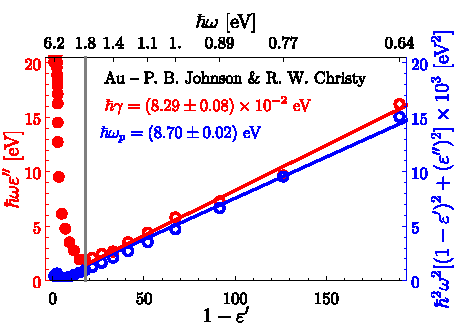
\includegraphics[scale=1]{1-Teoria/figs/1-4-DrudeFit_Au.pdf}
	\end{subfigure}
	\begin{subfigure}{.01\linewidth}\caption{}\label{sfig:FitDrudeAg}\vspace{3.75cm}\end{subfigure}
	\begin{subfigure}{.45\linewidth}\hspace*{-1em}
	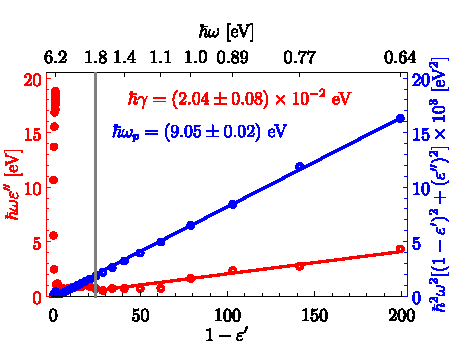
\includegraphics[scale=1]{1-Teoria/figs/1-4-DrudeFit_Ag.pdf}
	\end{subfigure}\vspace*{-.7em}
	\caption{ Determinación de los parámetros $\hbar\gamma$ (rojo) y $\hbar\omega_p$ (azul) mediante las Ecs. \eqref{eq:gammaAjuste} y \eqref{eq:omegaAjuste}, respectivamente, para los datos experimentales de la función dieléctrica \textbf{a)} del oro y \textbf{b)} la plata obtenidos de \cite{johnson1972constants}; la dependencia en la energía $\hbar\omega$ se muestra en la escala superior. Los círculos corresponden a datos considerados para el ajuste al modelo de Drude-Sommerfeld, mientras que los discos corresponden a los datos de contribuciones no plasmónicas; la división entre ambos regímenes corresponde a la línea vertical gris que para ambos casos se encuentra en $\hbar\omega\approx 1.76$ eV.}\label{fig:FitDrude}
	\end{figure}	

%	\begin{figure}[h!]\centering\hspace*{-1.5em}
%	\begin{subfigure}{.01\linewidth}\caption{}\label{sfig:sizeAu}\vspace{3.75cm}\end{subfigure}
%	\begin{subfigure}{.45\linewidth}\hspace*{-1.3em}
%	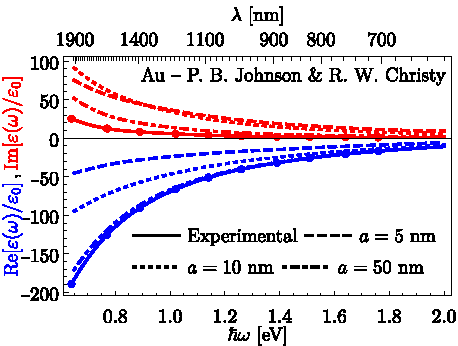
\includegraphics[scale=1]{1-Teoria/figs/1-4-sizeAuSmall.pdf}
%	\end{subfigure}
%	\begin{subfigure}{.01\linewidth}\caption{}\label{sfig:sizeAg}\vspace{3.75cm}\end{subfigure}
%	\begin{subfigure}{.45\linewidth}\hspace*{-1em}
%	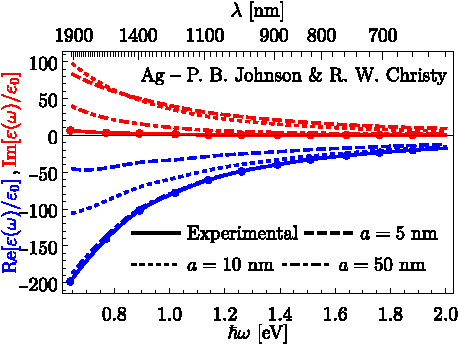
\includegraphics[scale=1]{1-Teoria/figs/1-4-sizeAgSmall.pdf}
%	\end{subfigure}\vspace*{-.7em}
%	\caption{ Comparación de la función dieléctrica como función de la energía $\hbar\omega$ para el\textbf{a)}  oro y \textbf{b)} la plata en bulto (líneas continuas) y para NPs esféricas de radio $a=5$ nm (líneas discontinuas), $a=10$ nm (líneas punteadas) y $a=50$ nm (líneas punto punteadas). La dependencia de la función dieléctrica con la longitud de onda $\lambda$ se muestra en el marco superior.}\label{fig:sizeCorrection}
%	\end{figure}	

%
%
%	\begin{figure}[h!]\centering
%	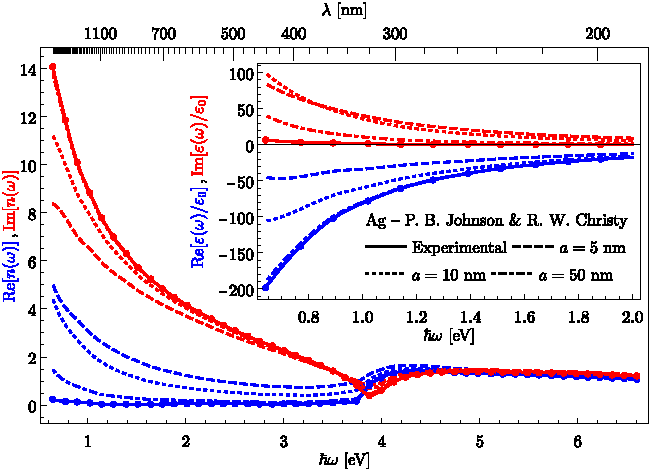
\includegraphics[scale=1]{1-Teoria/figs/0-sizeAgBig.pdf}
%    \vspace*{-1em}
%	\caption{ Comparación del índice de refracción (gráfica principal) y la función dieléctrica (gráfica secundaria) como función de la energía $\hbar\omega$ para el oro en bulto (líneas continuas) y para NPs esféricas de radio $a=5$ nm (líneas discontinuas), $a=10$ nm (líneas punteadas) y $a=50$ nm (líneas punto punteadas). La dependencia de la función dieléctrica con la longitud de onda $\lambda$ se muestra en el marco superior.}
%	\end{figure}		
%	
%	
%	\begin{figure}[h!]\centering
%	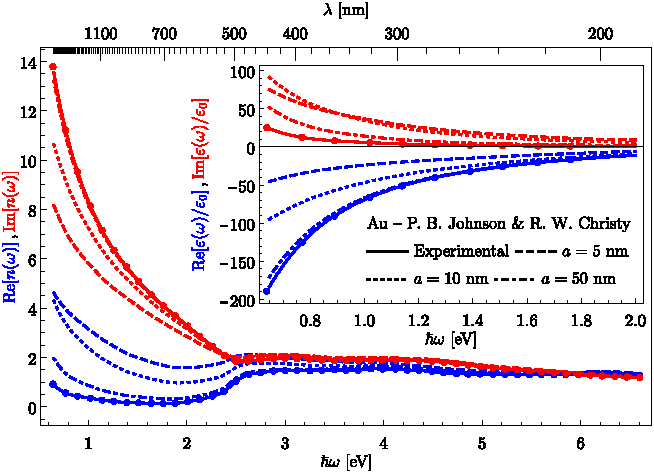
\includegraphics[scale=1]{1-Teoria/figs/0-sizeAuBig.pdf}
%    \vspace*{-1em}
%	\caption{Comparación del índice de refracción (gráfica principal) y la función dieléctrica (gráfica secundaria) como función de la energía $\hbar\omega$ para la plata en bulto (líneas continuas) y para NPs esféricas de radio $a=5$ nm (líneas discontinuas), $a=10$ nm (líneas punteadas) y $a=50$ nm (líneas punto punteadas). La dependencia de la función dieléctrica con la longitud de onda $\lambda$ se muestra en el marco superior.}
%	\end{figure}		

En la Fig.  \ref{fig:sizeCorrection} se muestra la correción por tamaño de la función dieléctrica del oro [Fig. \ref{sfig:sizeAu}] y la plata [Fig.  \ref{sfig:sizeAg}] para partículas esféricas, considerando $A=1$ en la Ec. \eqref{eq:sizeCorrection} \cite{noguez2007surface}. Tanto para el oro como para la plata, la función dieléctrica de bulto, experimental, corresponde a las líneas continuas y los puntos a sus valores experimentales; la función dieléctrica para NPs esféricas de radio $a=5$ nm corresponde a las líneas discontinuas; para $a=10$ nm, líneas punteadas; y para $a=50$ nm, líneas punto-discontinuas. Asimismo, para ambos materiales, la función dieléctrica para NPs se asemeja a la de bulto para energías $\hbar\omega>2$ eV. sin embargo, para $\hbar\omega<2$ eV, los efectos de tamaño son apreciables y más significativos mientras menor sea el radio de las NPs, como se observa tanto  en la parte real (líneas azules) como en la imaginaria (líneas rojas) de la función dieléctrica [ver ampliaciones en la Fig. \ref{fig:sizeCorrection}].

	\begin{figure}[h!]\centering\hspace*{-1.5em}
	\begin{subfigure}{.01\linewidth}\caption{}\label{sfig:sizeAu}\vspace{7cm}\end{subfigure}
	\begin{subfigure}{.7\linewidth}\hspace*{-1em}
	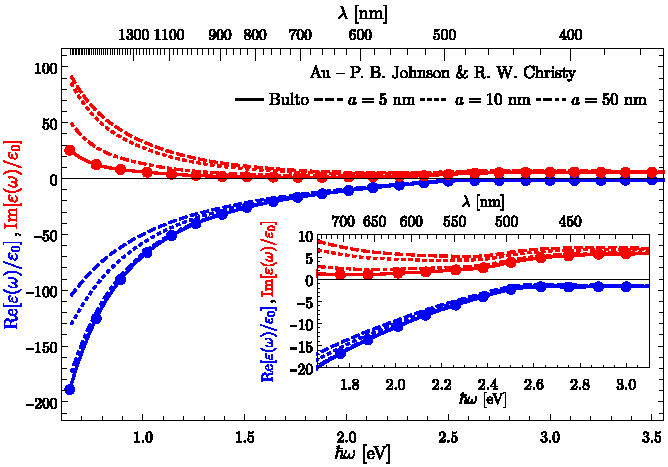
\includegraphics[scale=1]{1-Teoria/figs/0-sizeAuEpsilon.pdf}
	\end{subfigure}\\ \hspace*{-1.5em}
	\begin{subfigure}{.01\linewidth}\caption{}\label{sfig:sizeAg}\vspace{7cm}\end{subfigure}
	\begin{subfigure}{.7\linewidth}\hspace*{-1em}
	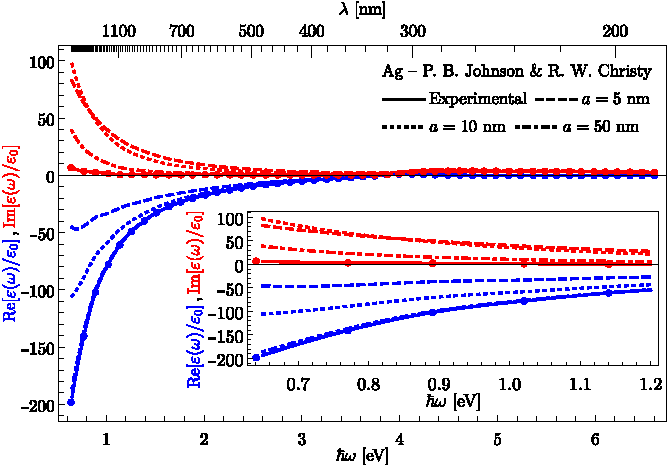
\includegraphics[scale=1]{1-Teoria/figs/0-sizeAgEpsilon.pdf}
	\end{subfigure}\vspace*{-.7em}
	\caption{Comparación de la función dieléctrica (parte real en azul e imaginaria en rojo) como función de la energía $\hbar\omega$ para \textbf{a)} el oro y \textbf{b)} la plata en bulto (líneas continuas) y para NPs esféricas de radio $a=5$ nm (líneas discontinuas), $a=10$ nm (líneas punteadas) y $a=50$ nm (líneas punto-discontinuas). La dependencia de la función dieléctrica con la longitud de onda $\lambda$ se muestra en la escala superior. Los datos experimentales para la función dieléctrica de bulto fueron tomados de \cite{johnson1972constants}, y se grafican como los puntos en \textbf{a)} y en \textbf{b)}.}\label{fig:sizeCorrection}
	\end{figure}	

\subsection{Plasmones}

En la deducción de la función dieléctrica del modelo de Drude [Ec. \eqref{eq:Drude}] se resolvió la ecuación de movimiento de los electrones libres en un material ante la  presencia de un campo eléctrico oscilante en el tiempo. A las oscilaciones colectivas (modos propios) de los electrones libres debido al acoplamiento con la radiación EM se les denominan  plasmones, que pueden ocurrir en el bulto \cite{stockman2011nanoplasmonics}, o bien, sobre una superficie. A diferencia del plasmón de volumen, las resonancias plasmónicas de superficie (Surface Plasmon Resonances, SPRs) pueden clasificarse en modos propagantes y localizados. Cuando un plasmón se propaga a lo largo de una interfaz plana entre un medio diel\'ectrico y uno met\'alico, se le denomina  \emph{plasm\'on-polarit\'on de superficie} (Surface Plasmon Polariton, SPP) \cite{maier2007plasmonics}.  Si el plasmón, en cambio, se encuentra en la superficie de una partícula  met\'alica, de tamaño finito, se le conoce como \emph{resonancia de plasm\'on de superficie localizado} (Localized Surface Plasmon Resonance, LSPR) \cite{maier2007plasmonics}. 

Para determinar a qué frecuencias se excitan los plasmones de volumen se calcula el rotacional de la ley de Faraday-Lenz y se sustituye el rotacional del campo magnético con la ley de Ampère-Maxwell, y  tras calcular su transformada de Fourier el resultado es \cite{maier2007plasmonics}
%
	\begin{align*}
	\vb{k}(\vb{k}\cdot\vb{E})-k^2\vb{E} =
			 -\frac{\varepsilon(\omega)}{\varepsilon_0}
			 \frac{\omega^2}{c^2}\vb{E},
	\end{align*}
%
donde se hace la distinción entre los casos de ondas transversales ($\vb{k}\cdot\vb{E}=0$), obteniendo la relación de dispersión
%
	\begin{align*}
	k^2 = \frac{\varepsilon(\omega)}{\varepsilon_0}  \frac{\omega^2}{c^2},
	\tag{\ref{eq:dispersion} \emph{bis}}\label{eq:TMode}		
	\end{align*}
%
y los casos con ondas longitudinales ($\vb{k}\cdot\vb{E}=kE$), en donde
%
	\begin{align}
	\varepsilon(\omega) = 0.
	\label{eq:LMode}
	\end{align}
%
Para obtener la relación de dispersión de un plasmón de volumen, se sustituye la función dieléctrica del modelo de Drude-Sommerfeld [Ec. \eqref{eq:Drude}], considerando el límite $\gamma\to 0$, en las Ecs. \eqref{eq:TMode} y \eqref{eq:LMode}, dando como resultado \vspace*{-.75em}\begin{subequations}
%
	\begin{tcolorbox}[title = Relación de dispersión del plasmón de volumen,  breakable, ams align ]
%	\omega &=  \sqrt{(ck)^2+\omega_p^2}, & \mbox{(Modo transversal)}
	k^2 &= \frac{\omega^2-\omega_p^2}{c^2}, 	& \mbox{(Modo transversal)}\\
	\omega&=\omega_p.							& \mbox{(Modo longitudinal)}
	\label{eq:volumePlasmon}
	\end{tcolorbox}\end{subequations}\vspace*{-.75em}\noindent
%
Dado que el plasmón de volumen es un modo longitudinal no puede acoplarse a ondas EMs transversales \cite{maier2007plasmonics}. Por otro lado, el SPP sí responde a ondas EM transversales y su relación de dispersión se calcula al considerar la geometría presentada en la Fig. \ref{fig:SPP}, en donde un haz de luz incide sobre una interfaz plana entre un medio dieléctrico, con una función dieléctrica $\varepsilon_1(\omega)>0$ y uno metálico con $\varepsilon_2(\omega)$, es decir, que cumpla con que $\Re[\varepsilon_2(\omega)]<0$, que en el modelo de Drude-Sommerfeld [Ec. \eqref{eq:Drude}] basta con que $\omega<\omega_p$.

\begin{figure}[h!]\centering
	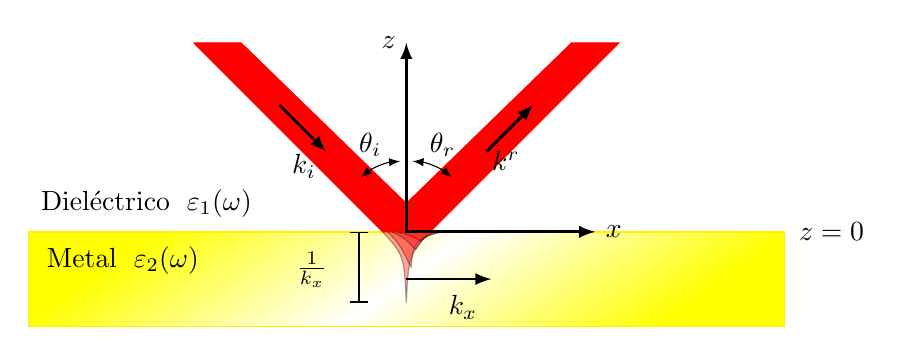
\begin{tikzpicture}[scale=1.2]
	%-------------------------------------------- Incidence media
\shadedraw[	top color = yellow,				%%%%	Color de arriba
			bottom color =yellow,				%%%%	Color de abajo
			middle color = white, 			%%	Color de en medio
			shading angle = 35]			%%%%	Ángulo de gradiente
		 (-4,-1) rectangle (4,0);
% Interface
\draw[yellow,line width=.5pt](-4,0)--(4,0)--(4,-1)--(-4,-1)--(-4,0); %%..5pt, interface]
% Media names
\node at (-2.75,.3) {Diel\'ectrico $\; \varepsilon_1(\omega)$}; 
\node at (-3,-.3) {Metal  $\; \varepsilon_2(\omega)$};
\node at (4.5,0) {$z=0$};

%-------------------------------------------- Laser beam outside
\draw[fill=red, opacity = 1,red](-2.25,2)--(-1.75,2)-- (0,.3)  %%% outside the metal
						--(1.75,2)--(2.25,2)
						--(.25,0)--(-.25,0)--(-2.25,2);																														
%--------------------------------------------  Incident Wave
\path (0,0)++(112.5:1cm)node{$\theta_i$};       % Angle
\draw[latex - latex](95:.75cm)arc(95:130:.75cm);
 
    \draw[- latex,line width=1pt](135:1.9cm)--(135:1.2cm);    %Wave vector
    \path (0,0)++(141:1.1cm)node[left]{$\vb{k}_i$};     %Wave vector label
    
%--------------------------------------------  Reflected Wave
\path (0,0)++(67.5:1cm)node{$\theta_r$};       % Angle
\draw[latex - latex](85:.75cm)arc(85:50:.75cm);
 
    \draw[- latex,line width=1pt](45:1.2cm)--(45:1.9cm);    %Wave vector
    \path (0,0)++(43:1.1cm)node[right]{$\vb{k}^r$};     %Wave vector label
  
%--------------------------------------------  Transmitted Wave & Skin depth
\draw[fill = red, opacity = .35] (-.25,0) ..controls (-.025,-.25) .. (0,-.75)
											..controls (.025,-.25) .. (.25,0);  %1st evanescent wave
\draw[fill = red, opacity = .35] (-.2,0) ..controls (-.075,-.125) .. (0.05,-.375)
											..controls (.075,-.125) .. (.3,0);  %2nd evanescent wave
\draw[fill = red, opacity = .35] (-.15,0) ..controls (-.025,-.0625) .. (0.1,-.1875)
											..controls (.175,-.0625) .. (.35,0);  %3rd evanescent wave
\draw[fill = red, opacity = .35] (-.1,0) ..controls (.025,-.03125) .. (0.15,-.09375)
											..controls (.225,-.03125) .. (.4,0);  %4th evanescent wave	

    \draw[- latex,line width=1pt](0,-.5)--(.9,-.5);    %Wave vector
    \node at (.6,-.8) {$\vb{k}_x$};
    
    \draw[|-|,line width=.2mm,black] (-.5,.0)--(-.5,-.75);%
    \node at (-1,-.4) {$\frac{1}{k_x}$};
%--------------------------------------------  Axes
\draw[latex - latex, line width =1pt] (0,2)node[left]{$z$}--(0,0) -- (2,0)node[right]{$x$};
\end{tikzpicture}
	\caption{ Esquema de una interfaz entre un medio dieléctrico ($z>0$) y uno metálico ($z<0$) sobra la que incide un haz de luz proveniente del medio dieléctrico; ambos  materiales son homogéneos, lineales e isótropos. La reflexión del haz de luz es total debido a la naturaleza metálica del material sin embargo, por las condiciones a la frontera de los campos EMs se presenta una onda evanescente en $z<0$ que se propaga en dirección de $\vb{k}_z$, paralela a la interfaz, la longitud de penetración de la onda evanecente es $1/k_x$, con $k_x$ la magnitud de $\vb{k}_x$. }\label{fig:SPP}
	\end{figure}
	
En la Fig. \ref{fig:SPP} se observa que al incidir el haz de luz sobre la interfaz ($z=0$)  entre el medio dieléctrico ($z>0$) y el metálico ($z<0$), se presenta una onda evanescente en el medio metálico que se propaga en la dirección de $\vb{k}_x=k_x\vu{e}_x$, cuya amplitud decae exponencialmente en la dirección $\vu{e}_z$ y cuyo máximo valor $1/k_x$ es su longitud de penetración. Si se considera que una onda plana, con frecuencia $\omega$ y vector de onda $\vb{k}^i$, es la que incide sobre la interfaz, los campos EMs de la onda evanescente se proponen como 

	\begin{subequations}\eqhalf{	\vb{E}(\vb{r},t) = \vb{E}(z)e^{ik_x x-\omega t },}
	\eqhalf{\vb{H}(\vb{r},t) = \vb{H}(z)e^{ik_x x-\omega t},}
	\label{eq:EHbetax}\end{subequations} \vspace*{-1em}
	
\noindent donde $\vb{E}(z>0)=\vb{E}_1$, con $E_1$ la magnitud del campo eléctrico dentro del dieléctrico, y $\vb{E}(z<0)=\vb{E}_2$ la magnitud del campo eléctrico en el medio metálico; lo análogo se cumple para el campo $\vb{H}$ y para la función dieléctrica $\varepsilon(z)$. La ecuación de Helmholtz [Ec. \eqref{eq:Helmholtz}] para los campos EMs de las Ecs. \eqref{eq:EHbetax} son

	\begin{subequations}
	\eqhalf{	\pdv[2]{\vb{E}}{z} + \qty[k_0^2\frac{\varepsilon(z)}{\varepsilon_0} - k_x^2 ] \vb{E}= 0,\label{eq:helmE}}
	\eqhalf{\pdv[2]{\vb{H}}{z} + \qty[k_0^2\frac{\varepsilon(z)}{\varepsilon_0}  - k_x^2 ] \vb{H}= 0, \label{eq:helmH}}
	\end{subequations} 
	
\noindent con $k_0 = \omega/c$. Para el cálculo de la relación de dispersión del SPP, se considera que existe homogeneidad en la dirección $y$, y que la única dependencia en la variable $x$  es en el término de propagación, es decir, que $\partial/\partial x\to ik_x$. Bajo estas consideraciones, al desarrollar la ley de Faraday-Lenz y la ley de Ampère-Maxwell con las expresiones de las Ecs. \eqref{eq:EHbetax}, se obtiene el siguiente conjunto de ecuaciones \vspace*{-1em}

	\begin{subequations}
	\eqhalf{	\mqty(-\pdv*{E_y}{z} \\ \pdv*{E_x}{z}-ik_x E_z\\ik_x E_y)
				= i\omega\mu_0 \mqty(H_x\\H_y\\h_z),}
	\eqhalf{	\mqty(-\pdv*{H_y}{z} \\ \pdv*{H_x}{z}-ik_x H_z\\ik_x H_y)
				= i\omega\varepsilon(z) \mqty(E_x\\E_y\\E_z).}	
	\end{subequations}\noindent 

El SPP es sensible a la polarización de la onda plana incidente por lo que se consideran los casos de polarización \emph{s} y \emph{p}. En polarización \emph{s}, las componentes no nulas de los campos EMs son $E_y$, $H_z$ y $H_x$, por lo que se  cumplen las relaciones

	\begin{subequations}
	\eqhalf{	H_x =  \frac{i}{\omega \mu_0} \pdv{E_y}{z},\label{eq:Hx}}
	\eqhalf{H_z =  \frac{k_x}{\omega \mu_0} E_y, \label{eq:Hz}}	
	\label{eq:ondaS}	\end{subequations} \vspace*{-1em}

\noindent junto con la ecuación de Helmholtz para el campo eléctrico [Ec. \eqref{eq:helmE}] con  $\vb{E} = E_y\vu{e}_y$, cuya solución se propone como
%
	\begin{align}
	E_y(z) = \begin{dcases}
		E_1 e^{ik_x x} e^{-k_{1,z}z}, & z>0\\
		E_2 e^{ik_x x} e^{k_{2,z} z}, & z<0
		\end{dcases},\label{eq:AnsatzEy}
	\end{align}
%	
con $k_{j,z} = k_j\cos\theta_i$ y $k_j = k_0 \sqrt{\varepsilon_j(\omega)/\varepsilon_0}$, con $j = 1,2$; donde se escribe de forma explícita el comportamiento de decaimiento exponencial en la amplitud y se omite el término $e^{-i\omega t}$ por simplicidad. Al calcular el campo $\vb{H}$ con las Ecs. \eqref{eq:ondaS} y \eqref{eq:AnsatzEy}, se obtienen a las expresiones 
	
	\eqhalf{	H_x(z) = \begin{dcases}
	-i \frac{E_1}{\omega\mu_0}k_{1,z} e^{ik_x x} e^{-k_{1,z} 	z}, & z>0\\
	i \frac{E_2}{\omega\mu_0}k_{2,z} e^{ik_x x} e^{k_{2,z} z}, & z<0
	\end{dcases},\notag}
	\eqhalf{	H_z(z) = \begin{dcases}
	\frac{E_1}{\omega\mu_0}k_x  e^{ik_x x} e^{k_{1,z} z} & z>0\\
	\frac{E_2 }{\omega\mu_0}k_x  e^{ik_x x} e^{k_{2,z}z} & z<0
	\end{dcases}.\notag}
	
\noindent   Las condiciones a la frontera impuestas en los campos EMs resultan en que las componentes paralelas a la interfaz del campo eléctrico, $E_y$, y del campo $\vb{H}$, $H_z$, sean continuas, por lo que $E_1 = E_2$. Adicionalmente, por la continuidad de la componente paralela a la interfaz del  campo $\vb{H}$, $H_x$, se concluye que en $z=0$
%
	\begin{align}
	E_1\qty(k_{1,z}+k_{2,z})= 0. \label{eq:condS}
	\end{align}
%
Por el \emph{Ansatz} propuesto en la Ec. \eqref{eq:AnsatzEy}, para que la onda evanescente esté confinada a la interfaz se debe cumplir que $k_{j,z}<0$, por tanto la Ec. \eqref{eq:condS} se satisface sólo si $E_1 = E_2 = 0$, es decir  que no existe un acoplamiento entre los electrones libres del metal en la interfaz plana y la onda EM incidente para polarización \emph{s}.

El cálculo de la relación de dispersión del SPP para polarización \emph{p} es análogo al cálculo con polarización \emph{s} al intercambiar el campo eléctrico por el campo $\vb{H}$ y al intercambiar la permeabilidad magnética por la función dieléctrica \cite{maier2007plasmonics}, es decir, $\vb{E}\leftrightarrow\vb{H}$ y $\varepsilon(z)\leftrightarrow\mu_0$. Al considerar las condiciones de continuidad del campo $\varepsilon(z)\vb{E}$ y el campo $\vb{H}$ se obtiene la expresión
%
	\begin{align*}
	\frac{E_1}{\omega}\qty( \frac{k_{1,z}}{\varepsilon_1}+  \frac{k_{2,z}}{\varepsilon_2} ) = 0,
	\end{align*}
%
de donde se obtiene que
%
	\begin{align}
	\frac{k_{1,z}}{k_{2,z}} = - \frac{\varepsilon_1}{\varepsilon_2}. \label{eq:condP}
	\end{align}
%
Asimismo, la ecuación de Helmholtz para el campo $\vb{H}$ [Ec. \eqref{eq:helmH}] impone que
%
	\begin{align}
	k_{j,z}^2 = k_x^2 - k_0^2 \frac{\varepsilon_j}{\varepsilon_0}.
	\label{eq:kdkm}
	\end{align}
%
Al elevar al cuadrado ambos lados de la Ec. \eqref{eq:condP}, sustituir $k_{j,z}^2$ con la Ec. \eqref{eq:kdkm}, y  despejar $k_x^2$  empleando la identidad de diferencia de cuadrados,  se calcula la relación de dispersión del SSP. Adicionalmente, como  $k_0^2 \varepsilon_j(\omega)= k_x^2 +k_{j,z}^2$, entonces \cite{maier2007plasmonics}\vspace*{-.75em}\begin{subequations}
%
	\begin{tcolorbox}[title = Relación de dispersión del SPP, breakable ]
	\eqhalf{k_x^2 = \frac{k_0^2}{\varepsilon_0} \frac{\varepsilon_1 \varepsilon_2}{\varepsilon_1 + \varepsilon_2},
	\label{eqs:kx}}
	\eqhalf{	k_{j,z}^2 = \frac{k_0^2}{\varepsilon_0} \frac{\varepsilon_j^2}{\varepsilon_1 + \varepsilon_2},\label{eqs:kz}}
	
	con $j=1$ para el medio dieléctrico y $j=2$ para el medio metálico.
	\end{tcolorbox}\label{eq:SPPRelDiso}\end{subequations}\vspace*{-.75em}\noindent
%	
Para que se obtenga una onda evanescente en la interfaz (modo ligado), $k_x$ debe ser una cantidad real y $k_z$ una cantidad imaginaria \cite{novotny2006principles}, por lo que en la Ec. \eqref{eqs:kx} la suma y el producto de las funciones dieléctricas deben ser ambas positivas o ambas negativas y $\varepsilon_1+\varepsilon_2<0$ en la Ec. \eqref{eqs:kz} \cite{novotny2006principles}, dando como resultado que $\varepsilon_1\varepsilon_2<0$. Estas condiciones se satisfacen con la suposición inicial en la que $\varepsilon_1$ corresponda a la respuesta EM de un medio dieléctrico y $\varepsilon_2$ a la de un metal \cite{novotny2006principles,maier2007plasmonics}. La frecuencia de resonancia $\omega$ del SPP se obtiene maximizando las Ecs. \eqref{eq:SPPRelDiso}, es decir, cuando $\varepsilon_1(\omega)+\varepsilon_2(\omega)$ es mínima. Si se emplea el modelo de Drude-Sommerfeld [Ec. \eqref{eq:Drude}] en el límite $\gamma\to 0$ para $\varepsilon_2(\omega)$, entonces \cite{maier2007plasmonics}  \vspace*{-.75em}
	\begin{tcolorbox}[title =Frecuencia de resonancia del SPP, ams align,  breakable ]
	\omega = \frac{\omega_p}{\sqrt{1+\varepsilon_1/\varepsilon_0}}.
	\end{tcolorbox}\vspace*{-.75em}\noindent

La Fig. \ref{fig:Relaciones_de_dispersion} muestra la relación de dispersión como la dependencia de la frecuencia $\omega$ con la componente paralela del vector de onda $k_x$, respecto a una interfaz entre el vacío ($\varepsilon_1=\varepsilon_0$) y un material descrito por le modelo de Drude-Sommerfeld [Ec. \eqref{eq:Drude}], en el límite $\gamma\to 0$ para una onda plana monocromática propagándose en el vacío (línea continua negra), para el plasmón de volumen (línea continua roja) y para un SPP (línea continua azul). Las líneas discontinuas roja y azul corresponden a los valores $\omega=\omega_p$ y $\omega=\omega_p/\sqrt{2}$, respectivamente, que son las frecuencias que delimitan el régimen de modos radiativos ($\omega>\omega_p$), donde las dos componentes del vector de onda $\vb{k}$ son cantidades reales, y el régimen de modos ligados ($\omega<\omega_p/\sqrt{2}$), donde $k_x$ es una cantidad real pero la componente del vector de onda perpendicular a la interfaz $k_z$ es una cantidad imaginaria. La línea discontinua negra corresponden a la relación de dispersión de una onda plana propagándose  en un medio con $n=1.5$.

\begin{figure}[h!]\centering
	\begin{tikzpicture}
	\node[inner sep=0pt] at (0,0)
    {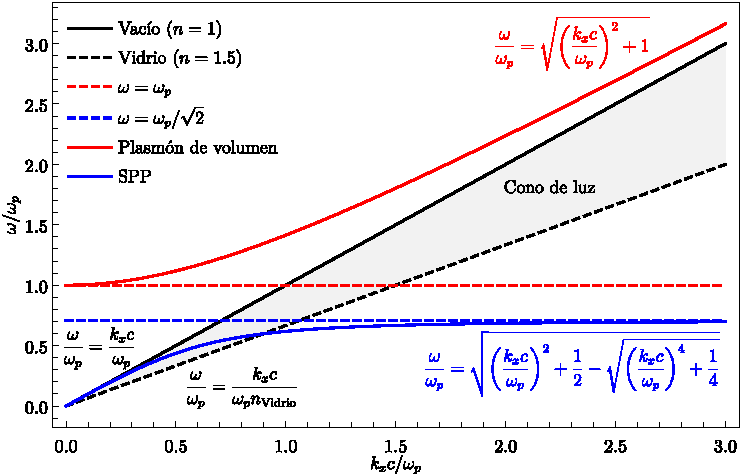
\includegraphics[scale=1]{1-Teoria/figs/1-4-RelacionDispersion.pdf}};
    \draw [thick, decorate, decoration={brace,amplitude=10pt,mirror}]
(6.5,-.8) -- (6.5,4.0);
\node at (8,2.5){\footnotesize Modo};
\node at (8,2.){\footnotesize radiativo};
\node at (8,1.5){\footnotesize $k_x\to\text{Real}$};
\node at (8,1.){\footnotesize $k_z\to\text{Real}$};
    \draw [thick, decorate, decoration={brace,amplitude=10pt,mirror}]
(6.5,-3.25) -- (6.5,-1.3);
\node at (8,-1.5){\footnotesize Modo};
\node at (8,-2.){\footnotesize ligado};
\node at (8,-2.5){\footnotesize $k_x\to\text{Real}$};
\node at (8,-3.){\footnotesize $k_z\to\text{Imaginario}$};
\end{tikzpicture}
\vspace*{-1em}
	\caption{Relación de dispersión en términos de $\omega/\omega_p$ como función de $k_xc/\omega_p$ de una onda plana monocromática en vacío (línea sólida negra), del plasmón de volumen (línea sólida roja) y del SPP (línea sólida azul) para materiales con una función dieléctrica tipo Drude en el límite $\gamma\to 0$, considerando una interfaz entre este material y el vacío ($\varepsilon_1 =\varepsilon_0$). El régimen de modos radiativos se encuentra en $\omega_p\leq\omega$ (igualdad denotada por la línea discontinua roja), donde $k_x$ y $k_z$ son cantidades reales; el régimen de modos ligados se encuentra en $\omega\leq\omega_p/\sqrt{2}$ (igualdad denotada por la línea discontinua azul), donde $k_x$ es una cantidad real pero $k_z$ es una cantidad imaginaria. Para excitar a un SPP es necesario cambiar el índice de refracción de la matriz, por ejemplo empleando un prisma para obtener una onda plana viajando en vidrio (línea punteada negra); la región sombreada delimita las frecuencias a las que el SPP puede excitarse.}
	\label{fig:Relaciones_de_dispersion}
	\end{figure}		

La relación dispersión de la onda plana monocromática propagándose en el vacío (línea continua negra en la Fig. \ref{fig:Relaciones_de_dispersion})  es igual a la del SPP (línea continua azul) para  $k_x=0$, por lo que no es posible excitar al SPP con este tipo de ondas \cite{trugler2011properties}. Sin embargo, es posible excitar al SPP empleando un tercer medio dieléctrico, con una función dieléctrica mayor al del dieléctrico que forma la interfaz con el medio metálico donde se excitará el SPP \cite{trugler2011properties}. Un método experimental, pero no el único \cite{maier2007plasmonics}, para excitar al SPP sobre la interfaz formada por una película delgada metálica con una función dieléctrica $\varepsilon_2(\omega)$ y la matriz, dieléctrico donde se encuentra inmersa la película, con $\varepsilon_1(\omega)$,  es emplear una configuración de reflexión total atenuada (Atenuatted Total Reflexión, ATR) \cite{kabashin2009plasmonic}, mostrada en la Fig. \ref{sfig:ATR}. En este tipo de configuración se emplea un tercer medio dieléctrico con función dieléctrica $\varepsilon_3(\omega)$ para generar una onda evanescente en la interfaz entre éste y la película delgada que logre penetrar hasta la interfaz entre la película delgada metálica y la matriz. En la Fig. \ref{fig:ATR-SPP} se muestra una posible arreglo para excitar experimentalmente al SPP. El arreglo consiste en una  película metálica, con una función dielétrica $\varepsilon_2(\omega)$ y altura $d$, inmersa en un dieléctrico $\varepsilon_1(\omega)=\varepsilon_0$ sobre un sustrato cuya función dieléctrica $\varepsilon_3(\omega)$ cumpla con $\varepsilon_3(\omega)>\varepsilon_1(\omega)$; en la Fig. \ref{sfig:ATR} el sustrato empleado es un prisma con $\varepsilon_3(\omega)/\varepsilon_0=1.5^2$. Cuando una onda plana monocromática incide sobre la interfaz entre la placa metálica y el sustrato, se produce una onda evanescente que se propaga en la dirección $\vb{k}_x=k_x\vu{e}_x$ y si $1/k_x>d$, la onda evanescente penetra la interfaz entre la matriz y la placa, excitando al SPP sobre la interfaz \cite{trugler2011properties}, representada por la línea naranja en la Fig. \ref{sfig:ATR}. En la Fig. \ref{sfig:SPP-R} se grafica la reflectancia $R$ como función del ángulo de incidencia $\theta_i$, de la longitud de onda $\lambda$ y la energía $\hbar\omega$, cuando una onda plana monocromática se propaga a través del prisma, con $\varepsilon_3(\omega)/\varepsilon_0 = 1.5^2$, e incide sobre una placa de oro de espesor $d=50$ nm inmersa en una matriz con $\varepsilon_1(\omega)/\varepsilon_0 = 1$. Para $\lambda<500$ nm la reflectancia es cercana a cero pues el oro se comporta como un dieléctrico, mientras que para $\lambda>500$ nm tiene una respuesta metálica por lo que la reflexión de luz aumenta; para $\theta_i>42^\circ$ la luz que incide sobre la placa metálica se refleja totalmente a excepción de una región resaltada por los puntos blancos, para la cual $R\approx 0$ en $\lambda>500$ nm, que  corresponde a las combinaciones de ángulo de incidencia y longitudes de onda ---equivalente a valores de $k_x$ y $\omega$, respectivamente-- a los que el SPP se propaga sobre la interfaz entre la placa de oro y el dieléctrico con $\varepsilon_1(\omega)/\varepsilon_0 = 1$.
			
	\begin{figure}[h!]\centering
	\begin{subfigure}{.01\linewidth}\caption{}\label{sfig:ATR}\vspace{5.5cm}\end{subfigure}
	\begin{subfigure}{.45\linewidth}\hspace*{-1.5em}
		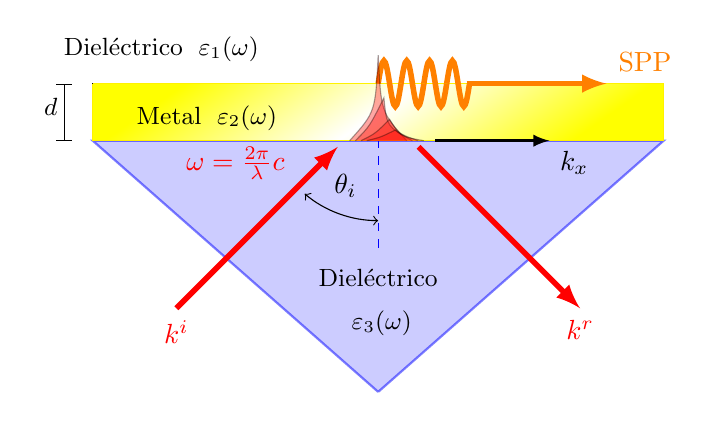
\begin{tikzpicture}[scale= 1.45]
	%-------------------------------------------- Incidence media
\def\a{.3}
\def\d{.3}
\def\dd{.2}
\def\l{2.5}
\def\ll{.05}

\fill[blue, opacity = .2] (0,-\l)--(\l,-\d)--(-\l,-\d);
\draw[blue, opacity = .5,thick] (0,-\l)--(\l,-\d)--(-\l,-\d)--(0,-\l);


\draw[|-|](-\l-.25,-\d)--(-\l-.25,+\dd);
\node at (-\l-.4,0) {\small $\;d$};
\draw[blue, dashed] (0,0)--(0,-\l*.5);

\path (0,0)++(-90-45*.5:\l*.3)node{$\theta_i$};       % Angle
\draw[<->](-90:\l*.4)arc(-90:-90-45*.89:\l*.4);

%\foreach \x in {-4,-2.9,-1,.1,1.2,2.4,3.8}{
%\fill[ball color=yellow, opacity=1] (\x,0) circle(\a);}

\shadedraw[	top color = yellow,				%%%%	Color de arriba
			bottom color =yellow,				%%%%	Color de abajo
			middle color = white, 			%%	Color de en medio
			shading angle = 35]			%%%%	Ángulo de gradiente
		 (-\l,-\d) rectangle (\l,\dd);
% Interface
\draw[yellow,line width=.5pt](-\l,\dd)--(\l,\dd)--(\l,-\d)--(-\l,-\d)--(-\l,\dd); %%..5pt, interface]

% Media names
\node at (0,-1.5) {\small Diel\'ectrico}; 
\node at (0,-1.9) {\small $\; \varepsilon_3(\omega)$}; 
\node at (-1.5,-.1) {\small Metal  $\; \varepsilon_2(\omega)$};
\node at (-1.9,.5) {\small Diel\'ectrico $\; \varepsilon_1(\omega)$}; 


\draw[latex -, thick, red, line width = 2](225:.5)--(225:2.5) node[anchor= north]{$\vb{k}^i$};
\node at (-1.25,-.5) {\color{red} $\omega =\frac{2\pi}{\lambda}c$};
\draw[- latex, thick, red, line width= 2](-45:.5)--(-45:2.5)node[anchor=north ]{$\vb{k}^r$};
\draw[- latex, thick,   line width = 1](.5,-\d)--(1.5,-\d) node[anchor= north west ]{$\vb{k}_x$};

\foreach \i in {0,4,8,12}{
\draw[thick, orange,line width = 2,] (\i*\ll,\dd) sin (\i*\ll+\ll,\dd*2) cos (\i*\ll+2*\ll,\dd) sin (\i*\ll+3*\ll,0) cos (\i*\ll+4*\ll,\dd);
}
\draw[- latex, thick, orange,  line width = 2](15.5*\ll,\dd)--(2,\dd) node[anchor= south west ]{SPP};



\draw[fill = red, opacity = .35] (-.25,-\d) ..controls (-.025,.25-\d) .. (0,.75-\d)
											..controls (.025,.25-\d) .. (.25,-\d);  %1st evanescent wave
\draw[fill = red, opacity = .35] (-.2,0-\d) ..controls (-.075,.125-\d) .. (0.05,.375-\d)
											..controls (.075,.125-\d) .. (.3,0-\d);  %2nd evanescent wave
\draw[fill = red, opacity = .35] (-.15,0-\d) ..controls (-.025,.0625-\d) .. (0.1,.1875-\d)
											..controls (.175,.0625-\d) .. (.35,0-\d);  %3rd evanescent wave
\draw[fill = red, opacity = .35] (-.1,0-\d) ..controls (.025,.03125-\d) .. (0.15,.09375-\d)
											..controls (.225,.03125-\d) .. (.4,0-\d);  %4th evanescent wave	


\end{tikzpicture}	
\end{subfigure}\hspace*{2em}
\begin{subfigure}{.01\linewidth}\caption{}\label{sfig:SPP-R}\vspace{5.5cm}\end{subfigure}
	\begin{subfigure}{.45\linewidth}\hspace*{-1em}
	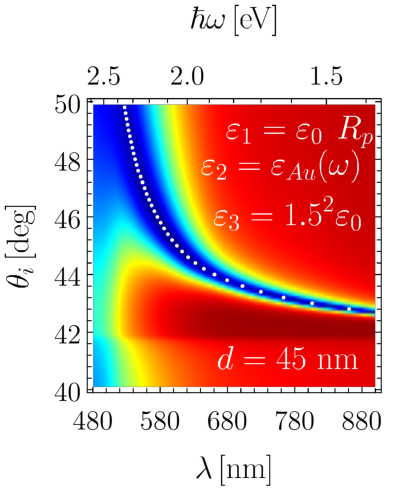
\includegraphics[scale=.85]{1-Teoria/figs/SPP.pdf}%
	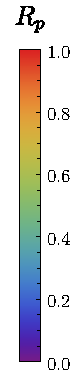
\includegraphics[scale=.73, trim={00 -40 00 00}, clip]{1-Teoria/figs/0-RBar_v}
	\end{subfigure}\hfill	\vspace*{-.7em}
	\caption{\textbf{a)} Esquema de una configuración ATR para la medición de la relación de dispersión del SPP mediante la reflectancia $R$ y \textbf{b)}  cálculo de la reflectancia al considerar una película de oro de espesor $d=50$ nm con una función dieléctrica $\varepsilon_2(\omega)$, dada por los datos experimentales de \cite{johnson1972constants}, inmersa en una matriz dieléctrica con $\varepsilon_1(\omega)/\varepsilon_0 = 1$ y sobre un prisma dieléctrico con $\varepsilon_3(\omega)/\varepsilon_0=1.5^2$. Cuando una onda plana monocromática con polarización \emph{p} incide sobre la interfaz entre el prisma y la película de oro a un ángulo mayor al crítico se produce una onda evanescente propagante en la dirección $\vb{k}_x=k_x\vu{e}_x$; si la longitud de penetración $1/k_x$ es mayor al espesor $d$ de la película metálica, es posible excitar al SPP sobre la interfaz entre el medio metálico y la matriz, como se observa en la Fig. \ref{fig:Relaciones_de_dispersion}. Los puntos blancos en \textbf{b)} corresponden a la relación de dispersión del SPP propagándose sobre la interfaz entre el aire y una película metálica de oro.}\label{fig:ATR-SPP}
	\end{figure}			
		
Los SPPs son ondas electromagnéticas propagantes acopladas a los electrones libres de un metal sobre una interfaz plana e infinita entre el metal y un medio dieléctrico \cite{maier2007plasmonics}. Cuando la interfaz  entre el medio metálico y el dieléctrico tiene una área finita, como sucede con NPs, el resultado de la interacción entre una onda plana incidente y los electrones libres del metal es una excitación no propagante, también causada por el acoplamiento entre la radiación EM y los electrones libres, denominada plasmón de superficie localizado (Localized Surface Plasmon, LSP) \cite{maier2007plasmonics}. La curvatura de las NPs tiene dos efectos en los LSPs: la amplificación de los campos EMs dentro y fuera de la NP (en límite de campo cercano) y la excitación del LSP con iluminación directa, es decir, 
sin emplear métodos como la iluminación en ATR u otros \cite{maier2007plasmonics}.

%Al considerar NPs esféricas, se puede emplear la solución de Mie para calcular los campos EMs incidentes ($\vb{E}^i$, $\vb{H}^i$), dados por las Ecs. \eqref{eq:EHiAEV}, los campos EMs esparcidos  por la NP ($\vb{E}^s$, $\vb{H}^s$), dados por las Ecs. \eqref{eq:EHsAEV} y \eqref{eq:MieCoef}, en términos de lo.
En presencia de una NP esférica iluminada por una onda plana monocromática, los campos EMs fuera de la NP corresponden a la suma de los campos EMs de la onda plana incidente ($\vb{E}^i$, $\vb{H}^i$) y de los campos EMs esparcidos por la NP ($\vb{E}^s$, $\vb{H}^s$), por lo que el vector de Poynting [Ec. \eqref{eq:Poynting}], al considerar su promedio temporal, puede escribirse como \cite{bohren1998absorption}
%
\begin{align*}
\langle\vb{S}\rangle_t 
		= \underbrace{\frac12 \Re \qty(\vb{E}^i\times\vb{H}^{i*})}_{\text{\normalsize $\langle\vb{S}^i\rangle_t $}} + 
		\underbrace{\frac12 \Re \qty(\vb{E}^s\times\vb{H}^{s*})}_{\text{\normalsize $\langle\vb{S}^s\rangle_t $}}+
		\underbrace{	\frac12 \Re\qty(\vb{E}^i\times\vb{H}^{s*} + \vb{E}^s\times\vb{H}^{i*})}_{\text{\normalsize$\langle\vb{S}^{ext}\rangle_t $}},
\end{align*}
%
en donde $\vb{S}^i$ y $\vb{S}^s$ son los vectores de Poynting correspondientes a la onda plana incidente, con número de onda $k_m$ y cuyo campo eléctrico tiene amplitud $E_0$, y a los campos EMs esparcidos por la NP, respectivamente, y $\vb{S}^{ext}$ corresponde a los productos cruzados. Le energía $W_{abs}$ trasportada por los campos EMs que es absorbida por la partícula se calcula al integrar $\langle\vb{S}\rangle_t$ sobre una esfera de radio $R$ concéntrica a la NP, cuyo radio sea mayor al radio de la NP, es decir,
%
\begin{equation}
W_{abs} = - \int_0^{2\pi}\int_0^{\pi}
		\qty(\langle\vb{S}^i\rangle_t +\langle\vb{S}^s\rangle_t 
				+\langle\vb{S}^{ext}\rangle_t )
		\cdot \vu{e}_r \,\dd a
		 = W_i-W_{sca}+W_{ext},
		 \label{eq:WaAll}
\end{equation}
%
donde $W_i = 0$, pues se asume que la matriz donde se encuentra inmersa la NP no es absorbente \cite{bohren1998absorption}. Como $W_{abs}$ es independiente de $R$, al suponer que tanto la matriz como la NP no son magnéticas, es posible emplear la solución de Mie para la expresión de $\vb{E}^s$ en el campo lejano dada por las Ecs. \eqref{eq:EHsFF} y a partir de ésta calcular $\vb{H}^s$ con ley de Faraday-Lenz [Ec. \eqref{seq:FLArm}], dando como resultado que $W_{sca}$ es \cite{bohren1998absorption}
%
 	\begin{equation}
W_{sca} = \frac{\pi\norm{E_0}^2}{\omega\mu_0 k_m}
		\sum_\ell^\infty (2\ell+1)\Re(-i\xi_\ell^*\xi_\ell')\qty(\abs{a_\ell}^2+\abs{b_\ell}^2),
	\label{eq:WsAll}
	\end{equation}
%
en donde $a_\ell$ y $b_\ell$ son los coeficientes de Mie [Ecs.  \eqref{eq:MieCoef}], $\xi_\ell(\rho) = \rho h_\ell^{(1)}(\rho)$ es una función de Riccati-Bessel, y donde además se emplearon las propiedades de ortogonalidad de las funciones $\sin\varphi$ y $\cos\varphi$ [Ec. \eqref{eq:ortSinCos}], de $\tau_\ell\pm\pi_\ell$ [Ec. \eqref{eq:ortTauPi}], junto con la relación \cite{bohren1998absorption}
%
	\begin{equation*}
	 \int_{-1}^{1}\qty[\pi_\ell(\mu)\pi_{\ell'}(\mu) + \tau_\ell(\mu)\tau_{\ell'}(\mu)]\dd\mu
 			= \delta_{\ell,\ell'} \frac{2\ell^2(\ell+1)^2}{2\ell+1}.
	 \end{equation*} 
%
Definiendo la función de Ricatti-Bessel $\chi_\ell (\rho) = -\rho y_\ell(\rho)$, se reescribe $\xi_\ell$ como $\xi_\ell= \psi_\ell-i\chi_\ell$, con $\psi_\ell(\rho) = \rho j_\ell(\rho)$. Dado que se cumple que $\chi_\ell\psi_\ell'-\psi_\ell\chi_\ell = 1$ \cite{bohren1998absorption}, y como $\psi_\ell$ y $\chi_\ell$ son funciones reales con variables reales, se obtiene que
%
\begin{equation*}
\Re(-i\xi_\ell^*\xi_\ell')=\Re\qty[(\chi_\ell^*\psi_\ell'-\psi_\ell^*\chi_\ell')
						-i(\psi\ell^*\psi_\ell'-\chi_\ell^*\chi_\ell') ] 
						= (\chi_\ell^*\psi_\ell'-\psi_\ell^*\chi_\ell') 
						= \chi_\ell\psi_\ell'-\psi_\ell\chi_\ell = 1.
\end{equation*}
%
Al sustituir $\Re(-i\xi_\ell^*\xi_\ell') = 1$ en la Ec. \eqref{eq:WsAll}, la energía transportada por los campos EMs esparcidos, por unidad de tiempo, es
%
\begin{equation}
W_{sca} = \frac{\pi\norm{E_0}^2}{\omega\mu_0 k_m}
		\sum_\ell^\infty (2\ell+1) \sum_\ell^\infty\qty(\abs{a_\ell}^2+\abs{b_\ell}^2) = I_i \frac{2\pi}{k_m^2}  \sum_\ell (2\ell+1) \qty(\abs{a_\ell}^2+\abs{b_\ell}^2),
\end{equation}
%
en donde $I_i = \norm{\langle\vb{S}^i\rangle} = \norm{E_0}^2k_m/2\omega\mu_0$ es la irradiancia, o energía por unidad de tiempo y unidad de área, transportada por la onda plana monocromática incidente. Al escribir los campos EMs incidentes en términos de las funciones $\pi_\ell$ y $\tau_\ell$, se calcula $W_{ext}$ de forma análoga a $W_{sca}$, obteniéndose
%
\begin{equation}
W_{ext} = I_i \frac{2\pi}{k_m^2}  \sum_\ell^\infty (2\ell+1) \Re(a_\ell + b_\ell).
\end{equation}
%

De la Ec. \eqref{eq:WaAll}, empleando las expresiones de $W_{sca}$ y $W_{ext}$, es posible calcular la energía absorbida $W_{abs}$ por la NP. Al despejar $W_{ext}$ de la Ec. \eqref{eq:WaAll} se obtiene que $W_{ext} = W_{abs}+W_{sca}$, razón por la que $W_{ext}$ es la energía que se extingue  mediante la absorción y esparcimiento de luz por la NP. Al normalizar $W_{sca}$ y $W_{ext}$ por la irradiancia de la onda plana incidente $I_i$, se obtienen cantidades con unidades de área, que se conocen como secciones transversales de extinción $C_{ext}$, absorción  $C_{abs}$ y esparcimiento $C_{sca}$ que se relacionan como \vspace*{-.75em}
%
	\begin{tcolorbox}[title = {Secciones transversales de extinción, absorción y esparcimiento}, breakable ]
	\begin{equation}
	C_{ext} = C_{abs} + C_{sca},
	\end{equation}	
	\eqhalf{C_{sca} = \frac{2\pi}{k_m^2}  \sum_\ell (2\ell+1) \qty(\abs{a_\ell}^2+\abs{b_\ell}^2),
	\label{eq:Cabs}}
	\eqhalf{C_{ext} = \frac{2\pi}{k_m^2}  \sum_\ell^\infty (2\ell+1) \Re(a_\ell + b_\ell), \label{eq:Cext}}

	con $a_\ell$ y $b_\ell$, los coeficientes de Mie, dados por la Ec. \eqref{eq:MieCoef}.
	\end{tcolorbox}\vspace*{-.75em} \noindent
%
Para poder comparar la cantidad de luz extinguida por partículas esféricas de distintos radios, se emplean las eficiencias de absorción $Q_{abs}$, esparcimiento $Q_{sca}$ y extinción $Q_{ext}$, que se calculan a través de las secciones transversales de absorción $C_{abs}$, esparcimiento $C_{sca}$ y extinción $C_{ext}$ al normalizarlas por la sección transversal geométrica de cada partícula $\pi a^2$, dando como resultado
%
\begin{equation}
\frac{C_{ext}}{\pi a^2} = \frac{C_{ext}}{\pi a^2}  + \frac{C_{ext}}{\pi a^2} 
\;\longrightarrow\; 	Q_{ext} = Q_{abs} + Q_{sca}.
\end{equation}
%
Para una NP esférica, la eficiencia de extinción $Q_{ext}$, al igual que los campos EMs esparcidos [Ec. \eqref{eq:EHsFF}],  está en términos de una expansión multipolar modulada por los coeficientes $a_\ell$ y $b_\ell$ [Ecs.  \eqref{eq:MieCoef}], que dependen, entre otros parámetros, de $N$ que es el cociente del índice de refracción de la partícula $n_p(\omega)$ y el de la matriz $n_m(\omega)$.  De la Ec.  \eqref{eq:Cext} se observa que, para un multipolo $\ell$ fijo, la contribución de los campos EMs en la extinción de luz es máxima  cuando  el denominador de los coeficientes de Mie es mínimo \cite{novotny2006principles,maier2007plasmonics}.  Si se considera que la respuesta óptica de la partícula es 	$\varepsilon_p (\omega) = n_p^2 (\omega)$, y se mantienen constantes el radio $a$ de la NP, el índice de refracción $n_m$ de la matriz y la longitud de onda $\lambda$ de la onda plana incidente, entonces a la frecuencia $\omega_\ell = c (2\pi / \lambda_\ell)$, donde el denominador de las Ecs.  \eqref{eq:MieCoef} es mínimo, se le denomina \emph{frecuencia del modo normal} de orden $\ell$ \cite{bohren1998absorption,maciel2017momentum}. Por ejemplo, los modos normales eléctricos ocurren a las frecuencias en las que $a_\ell$ es máximo, es decir, cuando 
%
	\begin{align}
	\psi_\ell(Nx)\xi_\ell'(x)-N\xi_\ell(x)\psi_\ell'(Nx) = 0. 
	\label{eq:an_resonance}
	\end{align}
%
Al considerar el límite de partícula pequeña ($x = k_m a\ll 1$) para esferas inmersas en vacío ($n_m=1$), haciendo un desarrollo en serie de Taylor de las funciones esféricas de Bessel y Hankel alrededor del origen y sustituyéndolas en la Ec.  \eqref{eq:an_resonance}, se obtiene que los modos normales eléctricos cumplen la relación \cite{maciel2017momentum}
%
	\begin{align}
	\varepsilon_p(\omega_\ell) = - \frac{\ell+1}{\ell}.  
	\label{eq:NormalModes}
	\end{align}
%
Si se emplea la función dieléctrica del modelo de Drude-Sommerfeld [Ec.  \eqref{eq:Drude}] y se sustituye en la Ec.  \eqref{eq:NormalModes}, al despejar $\omega_\ell$ tras considerar además el límite $\gamma\to 0$ y de partícula pequeña, la expresión para la frecuencia de resonancia del  modo normal del multipolo $\ell$ es \cite{maciel2017momentum}\vspace*{-.75em}
%
\begin{tcolorbox}[title =Frecuencia de resonancia del LSP, ams align,  breakable ]
	\frac{\omega_\ell}{\omega_p} = \sqrt{ \frac{\ell}{2\ell+1}}. \label{eq:PPequeña}
	\end{tcolorbox}\vspace*{-.75em}\noindent
%
Adicionalmente, si se considera la contribución de todos los órdenes multipolares ($\ell\to \infty$), la mayor frecuencia de resonancia es $\omega_\infty = \omega_p/\sqrt{2}$, que corresponde a la SPR de una esfera de radio infinito, equivalente a un plano infinito.

Para partículas esféricas de radio arbitrario $a$ con una función dieléctrica dada por el modelo de Drude-Sommerfeld, la frecuencia de resonancia $\omega_\ell$ sufre un corrimiento al rojo debido al tiempo de acomplamiento $a/c$ entre la interacción EM de la esfera y  la densidad de carga inducida que corresponde al plasmón de superficie \cite{aizpurua1998coupling}.  En la Fig.  \ref{fig:NormalModes} se muestran las frecuencias de resonancia $\omega_\ell$ normalizadas respecto a la frecuencia de plasma $\omega_p$, como función del parámetro adimensional $a\omega_p / c$ para los multipolos $\ell = 1,\,2,\,3,\,4$ y $5$. El límite de partícula pequeña [Ec.  \eqref{eq:PPequeña}]	se recupera cuando  $a\to 0$ (lado izquierdo de la gráfica en la Fig.  \ref{fig:NormalModes}).  

	\begin{figure}[h!]\centering
		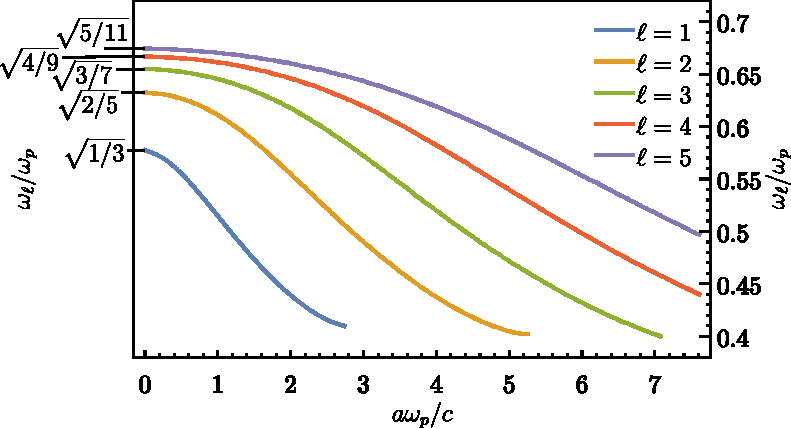
\includegraphics[scale=1]{1-Teoria/figs/1-4-DrudeMultipoles.pdf}\vspace*{-1em}
	\caption{Frecuencias de resonancia $\omega_\ell/\omega_p$ para una esfera con una función dieléctrica tipo Drude, como función del parámetro adimensional  $\omega_p a / c$, para los multipolos $\ell = 1,\,2,\,3,\,4$ y $5$. }
	\label{fig:NormalModes}
	\end{figure}		

Para una partícula esférica con una función dieléctrica arbitraria, los modos normales corresponden a las frecuencias en donde la sección transvesal de extinción es máxima para la contribución multipolar $\ell$ \cite{kreibig1995clusters}. En la Fig. \ref{fig:QextDrude} se grafica la eficiencia de extinción $Q_{ext}$ (línea continua azul) y la de esparcimiento $Q_{abs}$ (línea punteada azul) como función de la longitud de onda $\lambda$ y la energía $\hbar\omega$ para una partícula esférica de radio $a=30$ nm, inmersa en aire ($n_m=1$), con una función dieléctrica tipo Drude [Ec. \eqref{eq:Drude}] con los parámetros $\hbar\omega_p=4.3$ eV y $\hbar\gamma = 0.15$ eV [ver Fig. \ref{sfig:Qext4-30}] y con $\hbar\omega_p=10$ eV y $\hbar\gamma = 0.15$ eV [ver Fig. \ref{sfig:Qext10-30}].  Para determinar los modos normales del campo eléctrico en la partícula se grafican, adicionalmente, las contribuciones multipolares de las eficiencias de extinción $Q_{ext}^{(\ell)}$ para $\ell = 1,\,2$ y $3$, representadas por las líneas discontinuas verde, rosa y cian, respectivamente, en la escala vertical derecha. Cuando $\hbar\omega_p = 4.3$ eV, los modos normales, en términos de la longitud de onda, se excitan a $\lambda^{(1)}= 526$ nm, $\lambda^{(2)}= 462$ nm y $\lambda^{(3)}= 445 $ nm, mientras que para $\hbar\omega_p = 10$ eV se excitan a $\lambda^{(1)}= 265$ nm $\lambda^{(2)}= 211$ nm $\lambda^{(3)}= 195$ nm.

	\begin{figure}[h!]\centering\hspace*{-1.5em}
	\begin{subfigure}{.01\linewidth}\caption{}\label{sfig:Qext4-30}\vspace{3.75cm}\end{subfigure}
	\begin{subfigure}{.45\linewidth}\hspace*{-1.3em}
	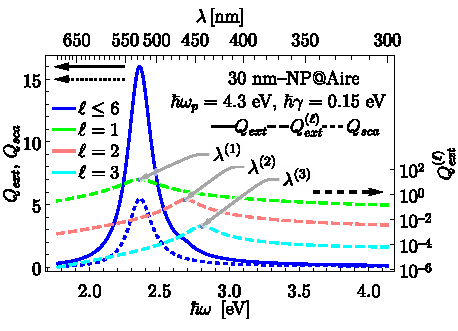
\includegraphics[scale=1]{1-Teoria/figs/1-5-Drude4-ExtSca_30.pdf}
	\end{subfigure}
	\begin{subfigure}{.01\linewidth}\caption{}\label{sfig:Qext10-30}\vspace{3.75cm}\end{subfigure}
	\begin{subfigure}{.45\linewidth}\hspace*{-1em}
	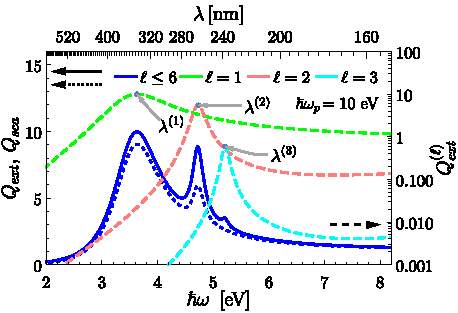
\includegraphics[scale=1]{1-Teoria/figs/1-5-Drude10-ExtSca_30.pdf}
	\end{subfigure}\vspace*{-.7em}
	\caption{Eficiencias de extinción $Q_{ext}$ (línea continua azul) y esparcimiento $Q_{sca}$ (línea punteada azul) como función de la energía $\hbar\omega$ para una partícula esférica con una función dieléctrica tipo Drude con los parámetros \textbf{a)} $\hbar\omega_p=4.3$ eV y $\hbar\gamma = 0.15$ eV y \textbf{b)} $\hbar\omega_p=10$ eV y $\hbar\gamma = 0.15$ eV; los resultados se obtuvieronal considerar la contribución de los primeros seis multipolos garantizando convergencia según el criterio de Wimcombe \cite{bohren1998absorption}. La contribución del multipolo $\ell$ en la eficiencia de extinción $Q_{ext}^{(\ell)}$ se grafica en escala logarítmica (eje vertical derecho) como función de la energía $\hbar\omega$ para localizar los modos normales; se consideraron los modos dipolares ($\ell =1$), cuadrupolares ($\ell = 2$) y octopolares ($\ell = 3$), correspondientes a las líneas verdes, rosas y azules, respectivamente.  Cuando $\hbar\omega_p = 4.3$ eV, los modos normales, en términos de la longitud de onda, se excitan a $\lambda^{(1)}= 526$ nm, $\lambda^{(2)}= 462$ nm y $\lambda^{(3)}= 445 $ nm, mientras que para $\hbar\omega_p = 10$ eV se excitan a $\lambda^{(1)}= 265$ nm $\lambda^{(2)}= 211$ nm $\lambda^{(3)}= 195$ nm.}
	\label{fig:QextDrude}
	\end{figure}	

Al considerar el caso con $\hbar\omega_p = 4.3$ eV, la extinción de luz a $2.3$ eV (modo dipolar) se debe no solo al esparcimiento, sino también a la absorción dado que $Q_{ext}>Q_{sca}$; un tercio de la extinción se debe al esparcimiento, y dos tercios a la absorción. De forma distinta, para $\hbar\omega_p = 10$ eV, el esparcimiento de luz predomina en el proceso de extinción de luz a $\hbar\omega= 4.7$ eV (modo dipolar).












